\section{The RationalGRL Framework}
\label{sect:overview}

Having explored the types of arguments and questions in requirements discussions, we now turn to an overview of our RationalGRL framework. We will show through a language definition and informal examples from our case study that it is possible to trace elements of the goal model back to their underlying arguments (\textbf{requirement 2}), and that it is possible to determine the effect of changes in the underlying argumentation on the goal model, and vice versa (\textbf{requirement 3}). A more formal, logical rendition of this traceability can be found in Section~\ref{sect:formalframework}.

The RationalGRL framework includes two parts: Argumentation and GRL goal modeling. The GRL part of RationalGRL allows for the creation of goal models by analyzing the non-functional requirements and refining the high-level goals into operationalized tasks. For the argumentation part, arguments and counterarguments can be put forward about various parts of this goal model. These two parts, GRL and argumentation, can impact the other side so that the models can be refined or new critical questions and argument schemes can be instantiated. For example, answering a critical question \emph{Is the task \emph{A} possible?} can result in removing or adding a task in the GRL model. Similarly,  if, for example, we add a new intentional element to the GRL model, it can lead to a new critical question relevant to this intentional element and its relationships.  

\begin{figure}[b]
\centering
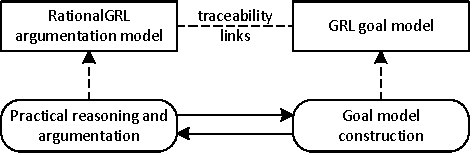
\includegraphics[width=\columnwidth]{img/framework.pdf}
\caption{The RationalGRL Framework}
\label{fig:rationalgrl-framework}
\end{figure}

\begin{table*}[t]
\centering
\begin{tabularx}{\textwidth}{|l|l|l|X|l|}
\hline
\multicolumn{2}{|c|}{\textbf{Argument scheme}} & \multicolumn{2}{c|}{\textbf{Critical Questions}} & \textbf{Effect}\\
\hline
AS0 & $a$ is an actor & CQ0 & Is the actor relevant? & \textsf{DISABLE} (no)\\
\hline
AS1 & Actor $a$ has resource $R$ & CQ1 &Is the resource available? & \textsf{DISABLE} (no)\\
\hline
AS2 & Actor $a$ can perform task $T$ & CQ2a &Is the task possible? & \textsf{DISABLE} (no)\\
&& CQ2b & Does the task have negative side-effects? & \textsf{DISABLE} (yes)\\
\hline
AS3 & Actor $a$ has goal $G$ & CQ3 & Can the desired goal be realized? & \textsf{DISABLE} (no)\\
\hline
AS4 & Actor $a$ has softgoal $S$ & CQ4 & Is the softgoal a legitimate softgoal?& \textsf{DISABLE} (no)\\
\hline
\hline
AS5 & Goal $G$ decomposes into task $T$ & CQ5a & Does the goal decompose into the task?& \textsf{DISABLE} (no)\\
& & CQ5b & Does the goal decompose into other tasks? & \textsf{INTRO} (yes)\\
 &  & CQ5c & Is the decomposition type correct? & \textsf{REPLACE} (no)\\
\hline
AS6 & Task $T$ contributes (negatively) to softgoal $S$& CQ6a & Does the task contribute to the softgoal?& \textsf{DISABLE} (no)\\
&& CQ6b & Are there alternative ways of contributing to the same softgoal?& \textsf{INTRO} (yes) \\
&& CQ6c & Does the task contribute (negatively) to some other softgoal?& \textsf{INTRO} (yes)\\
\hline
AS7 & Goal $G$ contributes to softgoal $S$ & CQ7a & Does the goal contribute to the softgoal?& \textsf{DISABLE} (no)\\
&& CQ7b & Does the goal contribute to some other softgoal?& \textsf{INTRO} (yes)\\
\hline
AS8 & Task $T$ depends on resource $R$ & CQ8 & Is the resource required in order to perform the task?& \textsf{DISABLE} (no)\\
\hline
AS9 & Actor $a$ depends on actor $b$ & CQ9 & Does the actor depend on any actors?& \textsf{INTRO} (yes)\\
\hline
AS10 & Task $T_i$ decomposes into task $T_j$ & CQ10a & Does the task decompose into the task? & \textsf{DISABLE} (no)\\
 &  & CQ10b & Does the task decompose into other tasks?& \textsf{INTRO} (yes)\\
 &  & CQ10c & Is the decomposition type correct? & \textsf{REPLACE} (no)\\
\hline
AS11 & Element $IE$ is relevant & CQ11 & Is the element relevant/useful? & \textsf{DISABLE} (no)\\
\hline
AS12 & Element $IE$ has name $n$ & CQ12 & Is the name clear/unambiguous? & \textsf{REPLACE} (no)\\
\hline
\hline
Att & Generic counterargument & Att & Generic counterargument & \textsf{DISABLE}\\
\hline
\end{tabularx}
\caption{List of argument schemes (AS0-AS13), critical questions (CQ0-CQ12), and the effect of answering them (right column).}
\label{table:argument-schemes}
\end{table*}


Figure~\ref{fig:rationalgrl-framework} presents an overview of RationalGRL framework. At the bottom there are two activities: \emph{practical reasoning \& argumentation} and \emph{goal model construction}. As already explained, these two activities influence each other: adding elements to a goal model gives rise to new critical questions about these elements, and answering critical questions with arguments may add or delete elements from the GRL model. The activities give rise to two different models: a \emph{RationalGRL model} (left-hand side) and a \emph{GRL model} (right-hand side). In the RationalGRL model, we have the goal model elements (goals, tasks etc) and the arguments for and against these elements; the GRL model contains only the goal model elements. Thus, the class of GRL models is essentially a subset of the class of RationalGRL models. Given the framework, it then becomes possible to trace a goal model back to the original argumentative discussion about goals, tasks and requirements. 

In the rest of this section, we discuss the individual parts of the GRL framework. In Section~\ref{sect:overview:as}, we continue our discussion of the argument schemes and critical questions for practical reasoning and argumentation, fitting these schemes and questions into our framework. In Section~\ref{sect:overview:lang}, we then discuss the language for RationalGRL models. In Section~\ref{sect:overview:examples}, we then provide extensive examples from our case study, illustrating the interplay between practical reasoning and argumentation on the one hand and RationalGRL models on the other hand.  

\subsection{The RationalGRL Argument Schemes and Critical Questions for Practical Reasoning}
\label{sect:overview:as}

A core aspect of the RationalGRL framework are the argument schemes, which should be close to the actual types of reasoning stakeholders or designers perform in the early requirements engineering phase (requirement 1 of our framework). Recall from section \ref{sect:gmas} that we ended up with a list of argument schemes and critical questions that were found in the transcripts (Table~\ref{table:transcripts:results:argumentschemes}). Using this list as a basis, we further refined our set of argument schemes and critical questions for RationalGRL into the list shown in Table~\ref{table:argument-schemes}. Note that this list of argument schemes and critical questions is not exhaustive. It is an initial list that we have obtained by coding transcripts. However, our framework is fully extensible, meaning that new argument schemes and critical questions can be added depending on the problem domain.

Schemes AS0-AS4 and AS12-AS13 are arguments for an element of a goal model, and AS5-AS11 are related to links in a goal model. The last scheme (Att) is a scheme for a generic counterargument against any type of argument that has been put forward. Arguments based on these schemes can be used to discuss a goal model. Making an argument based on one of the schemes effectively adds the corresponding GRL element to the model. See, for example, Table~\ref{table:transcripts:traffic-light} in Appendix~\ref{sect:transcripts:excerpts}: the participants argue for the addition of several tasks to the goal model using argument scheme AS2. 

An important part of arguing about goal models is asking the right critical questions. The critical questions presented in Table~\ref{table:argument-schemes} are therefore related to their respective argument schemes. These questions can be answered with ``yes'' or ``no'', and the type of answer has an effect on the original argument (\textsf{INTRO}, \textsf{DISABLE}, \textsf{REPLACE}). This will be further explained in Section~\ref{sect:overview:examples}. 

\subsection{The RationalGRL Modelling Language}
\label{sect:overview:lang}\label{sect:metamodel}
The language used to construct RationalGRL models is an extension of GRL: it includes all the GRL elements shown in Figure~\ref{fig:grl_legend}. However, there are also new elements corresponding to argumentation-related concepts. Figure~\ref{fig:rationalgrllegend} shows these elements. 
\begin{itemize}
\item \emph{Argument}: This represents an argument that does not directly correspond to a GRL element.  
\item \emph{Rejected (Disabled) GRL element}: If an argument or GRL element is attacked by an argument that itself is not attacked, then this GRL element will be rejected. 
%\item \emph{Refined GRL Element}: Not all critical questions attack a GRL element. It is also possible that a critical question \emph{replaces} an existing element (for instance, by clarifying the name of the element), or that it leads to the \emph{introduction} of a new element. In these cases, the corresponding GRL element is shown with a striped background. %%Refined GRL elements are not in the metamodel and the tool also has no different picture for refined elements
\item \emph{Attack Link}: An attack link can occur between an argument and another argument or GRL element. It means that the source argument attacks the target argument or GRL element.
\end{itemize} 

\begin{figure}[t]
\centering
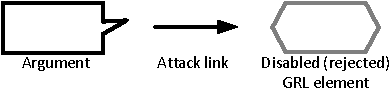
\includegraphics{img/legend.pdf}
\caption{The new elements and link of RationalGRL}
\label{fig:rationalgrllegend}
\end{figure}

The complete metamodel of the language can be found in Figure~\ref{fig:metamodel}. This metamodel represents the abstract grammar of the language, independently of the notation. The metamodel also formalizes the GRL concepts and constructs introduced in Section~\ref{sect:background:grl}\footnote{Note that for readability, some GRL concepts, such as contribution strength, have been omitted from the figure.}.

The metamodel consists of two packages, \emph{practical reasoning \& argumentation} and \emph{goal model construction}, which correspond to the relevant activities in the RationalGRL framework (cf. Figure~\ref{fig:rationalgrl-framework}). The goal model construction package consists of \textsf{GRLModelElements}, which can be either \textsf{GRLLinkableElements} or \textsf{ElementLinks}. A \textsf{GRLLinkableElement} can again be specialized into an \textsf{Actor} or an \textsf{IntentionalElement} (which is either a \textsf{Softgoal}, \textsf{Goal}, \textsf{Task}, \textsf{Resource}, or a \textsf{Belief}). Intentional elements can be part of an actor, and \textsf{GRLLinkableElements} are connected through \textsf{ElementLinks} of different types (i.e., \textsf{Contribution, Decomposition}, or \textsf{Dependency}). Finally, a \textsf{GRLmodel} is composed of \textsf{GRLModelElements}.

\begin{figure*}[t]
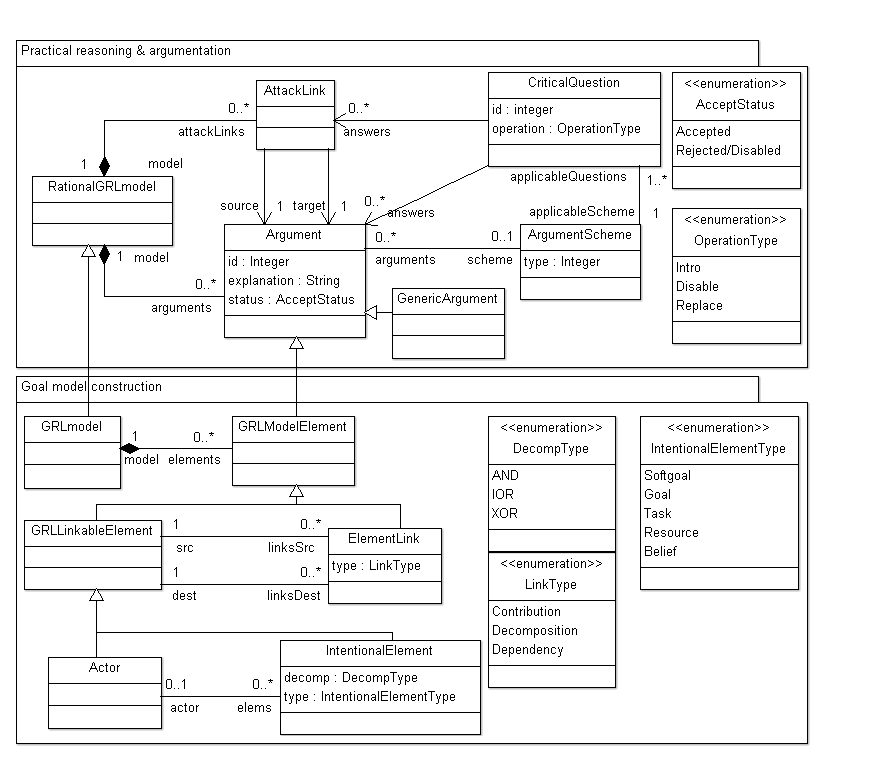
\includegraphics[width=\textwidth]{metamodel/metamodel}
\caption{The RationalGRL metamodel}
\label{fig:metamodel}
\end{figure*}

The practical reasoning and argumentation package depicts the concepts we introduced in Section~\ref{sect:overview:as}. An \textsf{ArgumentScheme} represents a scheme containing variables. \textsf{CriticalQuestions} are possible ways to attack or elaborate an argument based on a scheme; each critical question applies to exactly one scheme, but for each scheme there may be more than one applicable critical question. When an argument scheme is instantiated, we obtain an \textsf{Argument}. Therefore, each argument is associated with exactly one scheme, but a scheme can be instantiated in multiple ways. When a critical question is answered, we may obtain an \textsf{AttackLink}, an \textsf{Argument} or both, depending on the answer. Note that it is also possible to an \textsf{AttackLink} can also be associated with no critical questions. This allows the user to create attacks between arguments, which do not necessarily correspond to one of the critical questions. A \textsf{RationalGRLmodel} is composed out of arguments and attack relations.

Notice that there are various \textsf{OperationTypes} in the Argumentation package. In RationalGRL, these operations are performed by instantiating an argument scheme or answering a critical question in a certain way. An \textsf{INTRO} operation introduces a new RationalGRL element. A \textsf{DISABLE} operation creates a new argument that attacks another argument or GRL element, effectively disabling it. The \textsf{REPLACE} operation replaces a RationalGRL element with a new element. Instantiating an argument scheme from Table~\ref{table:argument-schemes} always leads to an \textsf{INTRO} operation, that is, it always introduces a new RationalGRL element. Answering a critical question can have different effects depending on the critical question and the answer. Table~\ref{table:argument-schemes} shows these effects for the different critical questions and answers. For example, answering CQ0 with ``no'' disables the argument based on AS0. 

There are two important links between the \emph{practical reasoning \& argumentation} and \emph{goal model construction} packages. First, each \textsf{GRLModelElement} is an \textsf{Argument}. This means that each model element inherits the \textsf{AcceptStatus} as well, allowing GRL elements to be accepted or rejected. This, furthermore, means that argument schemes can be applied to all GRL elements, capturing the intuition that each GRL element can be regarded as an instantiated argument scheme. Note that besides arguments about elements of the GRL model, we also have a \textsf{GenericArgument} which is simply a counter-argument to an existing argument that does not relate to any of the GRL elements. Finally, the relation between \textsf{GRLModelElement} and \textsf{Argument} means that, as we already briefly indicated when discussing the framework in Figure~\ref{fig:rationalgrl-framework}, the class of \textsf{RatinalGRLmodel} is a superclass of \textsf{GRLmodel}: besides arguments about GRL elements, we can also have arguments that does not relate to any of the GRL elements.

\subsection{From Practical Reasoning to RationalGRL Models: examples from the case study}
\label{sect:overview:examples}

We now turn to the interactions between the \emph{practical reasoning \& argumentation} (i.e. the bottom left element of the framework in Figure~\ref{fig:rationalgrl-framework}) on the one hand, and \emph{RationalGRL models} (i.e. the top left element of the framework in Figure~\ref{fig:rationalgrl-framework}) on the other hand. We provide informal examples of the links between the practical reasoning found in our case study transcripts and RationalGRL models. The formal grounding for the connection between practical reasoning and RationalGRL models can be found in the RationalGRL Metamodel (Section~\ref{sect:metamodel}) and in more detail in the logical formalization of the Argument Schemes and Critical Questions (Section~\ref{sect:algorithms}). The connection between the RationalGRL models shown in this section and regular GRL models is further formally defined in section \ref{sect:rationalGRL-GRL}. 

\paragraph{Example 1 - Introducing GRL elements with arguments (\textsf{INTRO)}}

\begin{figure}[t]
\centering
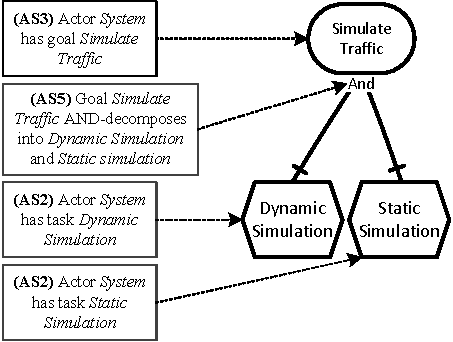
\includegraphics[width=\columnwidth]{img/fig_example_AS.pdf}
\caption{Introducing new GRL elements with argumentation (\textsf{INTRO)}.}
\label{fig:example_AS}
\end{figure}

We start by showing how instantiating argument schemes leads to the introduction of new RationalGRL elements in a model. Take the example in Figure~\ref{fig:example_AS}, which is based on the transcript excerpt shown in Table~\ref{table:transcript:decomposition}. On the left side, the arguments found in the transcript are shown, together with the argument scheme they are based on. The participants in the discussion argue that \emph{System} has a goal and two tasks, and that the goal AND-decomposes into the two tasks. By arguing in this way, new GRL elements are introduced. These GRL elements are shown on the right side of Figure~\ref{fig:example_AS}; the dashed arrows indicate the links between the practical reasoning and argumentation on the left and the RationalGRL model on the right. 


\paragraph{Example 2: Disabling GRL elements by answering critical questions (\textsf{DISABLE)}}

\begin{figure}[b]
\centering
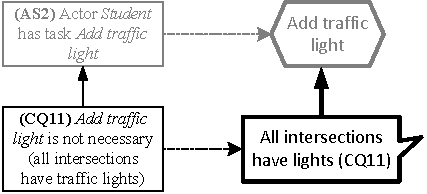
\includegraphics[]{img/fig_example_disable.pdf}
\caption{Disabling GRL tasks with argumentation (\textsf{DISABLE)}.}
\label{fig:example_disable}
\end{figure}

The transcript excerpt of this example is shown in Table~\ref{table:transcripts:traffic-light} in Appendix~\ref{sect:transcripts:excerpts} and comes from transcript $t_1$. In this example, participants first sum up functionality of the traffic simulator, which can be captured as instantiations of AS2. On left side of Figure~\ref{fig:example_disable} one such instantiation is shown, which leads to the addition of the task \emph{Add traffic light} in the RationalGRL model on the right side of Figure~\ref{fig:example_disable}. However, participant P1 notes that the problem description states that all intersections have traffic lights by default, so the task \emph{Add traffic light} is not necessary. This is captured using critical question CQ11. A negative answer to this question (cf. Table~\ref{table:argument-schemes}) should disable the original argument based on AS2 by attacking it. On the left side of Figure~\ref{fig:example_disable} a new argument (CQ11) attacks the original argument based on (AS2). This new argument is also added to the RationalGRL model on the right of Figure~\ref{fig:example_disable}, where it attacks the original task \emph{Add traffic light}. This attack leads to the original argument being \emph{rejected} (cf. Section~\ref{sect:background:pras} and Section~\ref{sect:goalmodeling:argumentationsemantics}), indicated by it being greyed out. As a result of this, the corresponding GRL task \emph{Add traffic light} is also disabled. 

\paragraph{Example 3: Changing a decomposition type by answering critical questions (\textsf{REPLACE})} 

\begin{figure}[t]
\centering
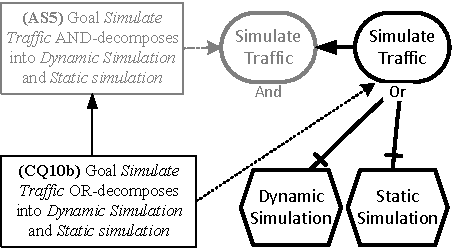
\includegraphics[]{img/fig_example_replace.pdf}
\caption{Replacing a GRL decomposition with argumentation (\textsf{REPLACE)}.}
\label{fig:examples:decomposition}
\end{figure}

The transcript excerpt of this example is shown in Table~\ref{table:transcript:decomposition} in the appendix and comes from transcript $t_3$. It consists of a discussion about the type of decomposition relationship for the goal \emph{Simulate Traffic}. Recall that in Example 1, an AND-decomposition was introduced for this goal with AS5 (Figure~\ref{fig:example_AS}). In the discussion CQ10b -- ``Is the decomposition type correct?'' -- is explicitly asked. The answer is ``No, it should be OR''. The original argument for AND-decomposition is now attacked  by the argument for the OR-decomposition, and the new argument is linked to the OR-decomposition in the RationalGRL model (Figure~\ref{fig:examples:decomposition}). 

\paragraph{Example 4: Clarifying a task by answering critical questions (\textsf{REPLACE})}

The transcript excerpt of this example is shown in Table~\ref{table:transcript:task-clarification} in Appendix~\ref{sect:transcripts:excerpts} and comes from transcript $t_1$. The discussion starts with an instantiation of argument scheme AS2: ``Actor \emph{Student} has task \emph{Set car influx}''. This argument is then challenged with critical question CQ12: ``Is the task \emph{Set car influx} specific enough?''. This is answered negatively, creating a new argument ``Actor \emph{Student} has task \emph{Set car influx per road}'', which attacks the original argument for \emph{Set car influx}. Note how the new task \emph{Set car influx per road} also attacks (and disables) the original RationalGRL task \emph{Set car influx} (Figure~\ref{fig:examples:clarification}). 

\begin{figure}[b]
\centering
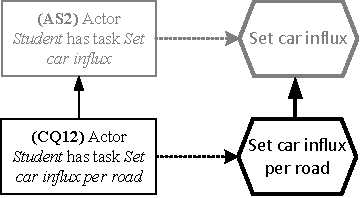
\includegraphics[]{img/fig_example_rename.pdf}
\caption{Renaming a GRL task with argumentation (\textsf{REPLACE)}.}
\label{fig:examples:clarification}
\end{figure}

\paragraph{Example 5: Defending the addition of an actor (\textsf{DISABLE)}}

\begin{figure}[t]
\centering
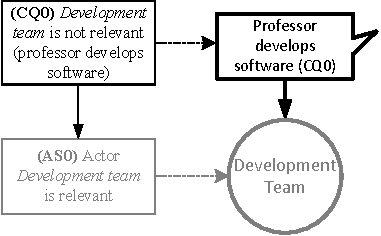
\includegraphics[]{img/reinstate1.pdf}
\caption{Disabling a GRL actor with argumentation (\textsf{DISABLE)}.}
\label{fig:examples:relevant-actor}
\end{figure}

The transcript excerpt of this example is shown in Table~\ref{table:transcript:irrelevant-actor} in the appendix and comes from transcript $t_3$. First participant \emph{P1} puts forth the suggestion to include actor \emph{Development team} in the model. This is, then, questioned by participant \emph{P2}, who argues that the professor will develop the software, so there will not be any development team. This is shown in Figure~\ref{fig:examples:relevant-actor}: first the actor \emph{Development Team} is introduced with an argument based on AS0. This argument is then attacked by answering critical question CQ0. 

\begin{figure}[t]
\centering
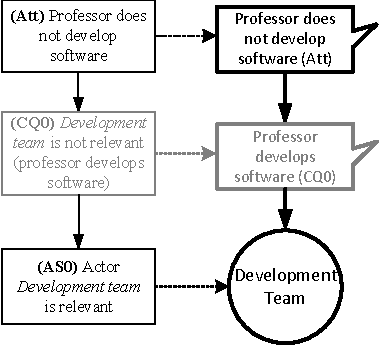
\includegraphics[]{img/reinstate2.pdf}
\caption{Defending a GRL actor by attacking its disabling attacker (\textsf{DISABLE)}.}
\label{fig:examples:relevant-actor2}
\end{figure}

Further in the discussion, participant \emph{P2} argues that the development team should be considered, since the professor does not develop the software. This is captured using a generic counterargument (\emph{Att} in Table~\ref{table:argument-schemes}), which attacks the earlier argument based on CQ0. Figure~\ref{fig:examples:relevant-actor2} shows the situation after the counterargument has been put forward: the argument (Att) now attacks the argument (CQ0), which in turn attacks the original argument (AS0). As a result, the argument (AS0) is acceptable (cf. Section~\ref{sect:background:pras} and Section~\ref{sect:goalmodeling:argumentationsemantics}), which causes the actor in the RationalGRL model to be enabled again.

